\documentclass[border=10pt]{standalone}

\usepackage{tikz}
\usepackage{tikzsymbols}
\usetikzlibrary{calc,patterns,shapes.geometric}

\def\centerarc[#1](#2)(#3:#4:#5){\draw[#1] ($(#2)+({#5*cos(#3)},{#5*sin(#3)})$) arc (#3:#4:#5);}

\begin{document}
	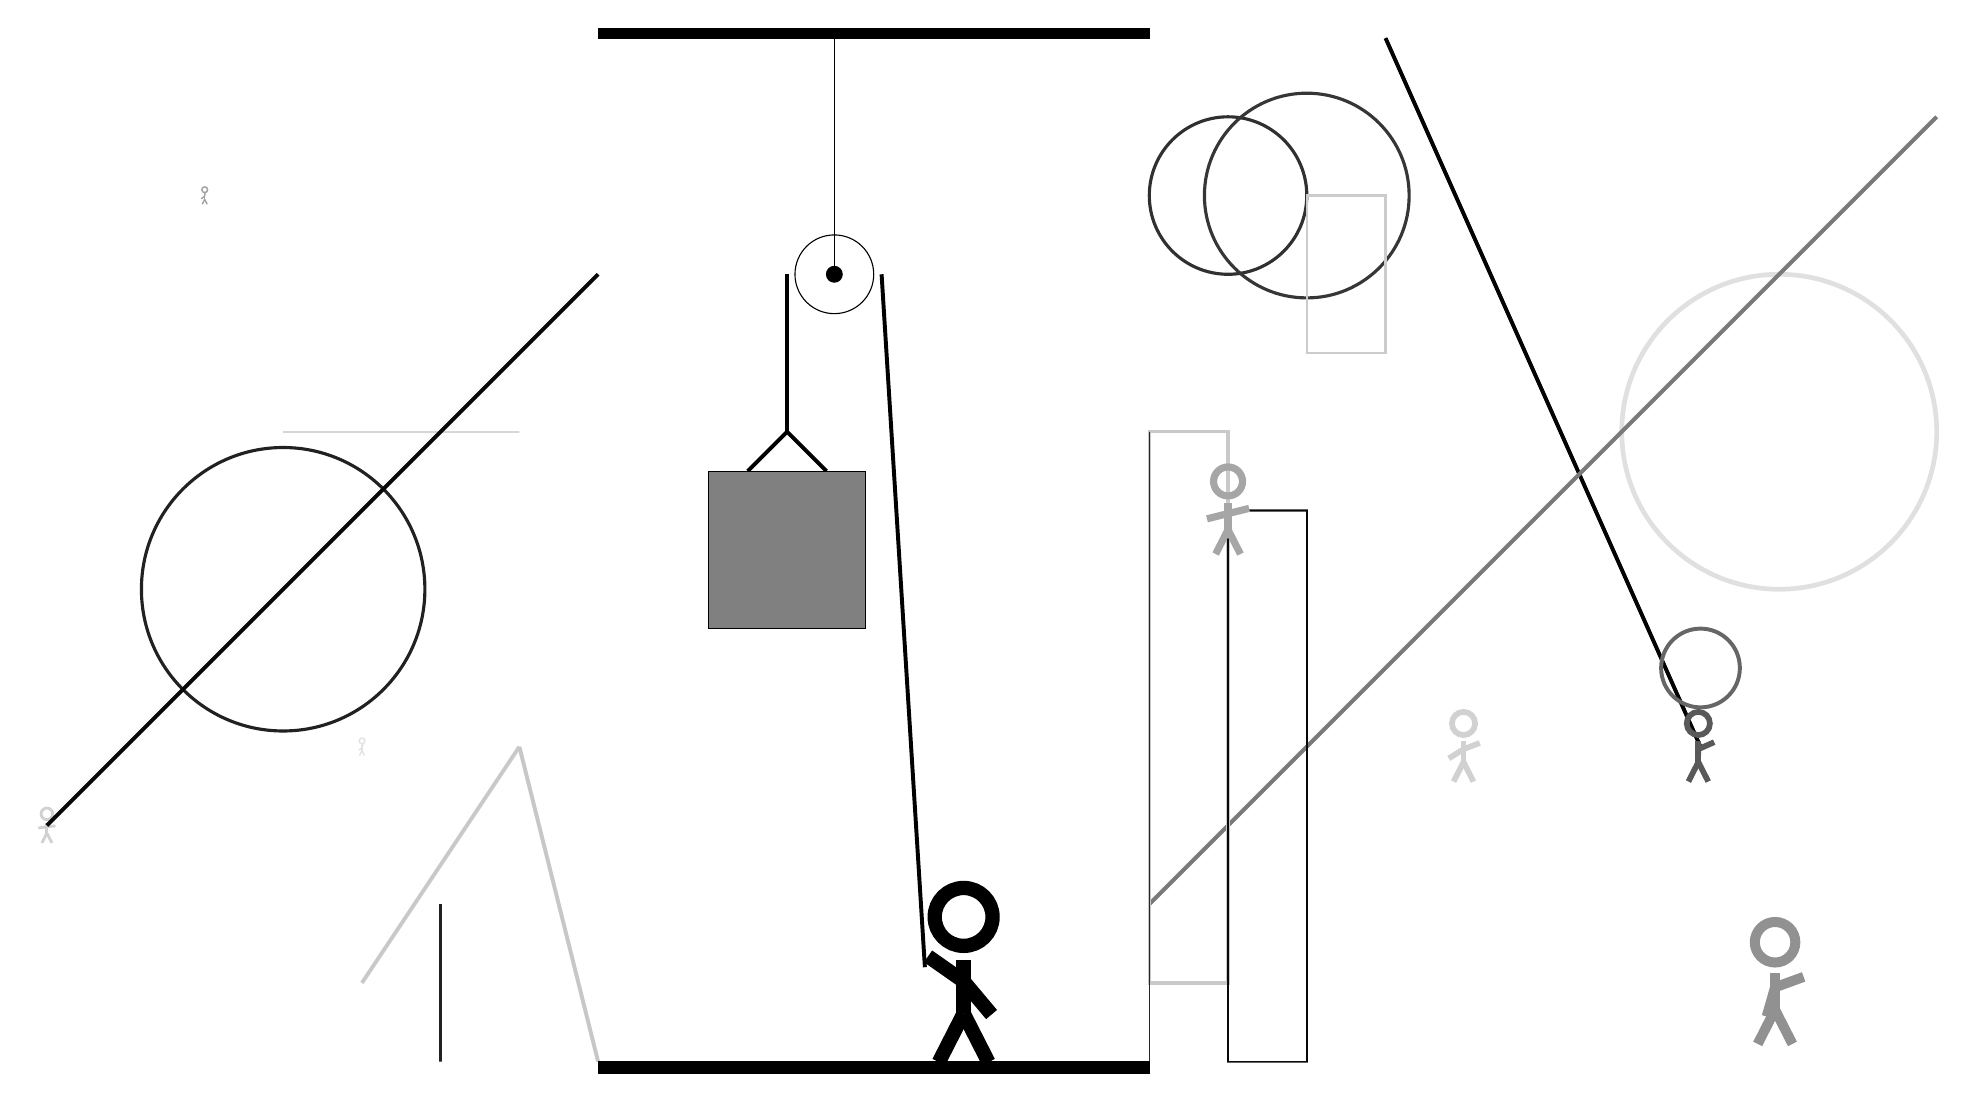
\begin{tikzpicture}
		%%%%% START %%%%%
		
		\draw[fill=black] (-2, 10) rectangle (5, 10.125);
		
		\draw (1, 7) circle (0.5);
		\draw[fill=black] (1, 7) circle (0.1);
		\draw (1, 10) -- (1, 7);
		
		\node[line width=0.4mm, color=black!18] at (-9, 0) {\Strichmaxerl[2][9][5]};
		
		\draw [line width=0.4mm, color=black!87](-6, 3) circle (1.8);
		\draw[line width=0.2mm, color=black!16] (-3, 5) rectangle (-6, 5);
		\draw [line width=0.6mm, color=black!12](13, 5) circle (2.0);
		\draw [line width=0.3mm, color=black!64](7, 9) circle (0.0);
		\draw [line width=0.4mm, color=black!81](6, 8) circle (1.0);
		\node[line width=0.4mm, color=black!43] at (13, -2) {\Strichmaxerl[7][74][20]};
		\draw [line width=0.7mm, color=black!31](9, 5) circle (0.0);
		\draw[line width=0.5mm, color=black!99](8, 10) -- (12, 1);
		\draw[line width=0.5mm, color=black!52](5, -1) -- (15, 9);
		\draw[line width=0.5mm, color=black!97](-2, 7) -- (-9, 0);
		\draw [line width=0.4mm, color=black!79](7, 8) circle (1.3);
		\draw [line width=0.5mm, color=black!60](12, 2) circle (0.5);
		
		\draw[line width=0.4mm, color=black!21] (5, -2) rectangle (6, 5);
		\node[line width=0.3mm, color=black!65] at (12, 1) {\Strichmaxerl[4][88][24]};
		\draw[line width=0.3mm, color=black!20] (7, 8) rectangle (8, 6);
		
		\draw[line width=0.3mm, color=black!61] (6, -3) rectangle (7, 4);
		\draw[line width=0.5mm, color=black!21](-5, -2) -- (-3, 1);
		\draw[line width=0.3mm, color=black!87] (-4, -1) rectangle (-4, -3);
		\draw[line width=0.5mm, color=black!22](-2, -3) -- (-3, 1);
		\draw[line width=0.4mm, color=black!79] (5, 9) rectangle (5, 9);
		\draw[line width=0.2mm, color=black!97] (7, 4) rectangle (6, -3);
		\node[line width=0.3mm, color=black!11] at (-5, 1) {\Strichmaxerl[1][43][72]};
		\node[line width=0.7mm, color=black!18] at (9, 1) {\Strichmaxerl[4][32][21]};
		\node[line width=0.7mm, color=black!37] at (-7, 8) {\Strichmaxerl[1][37][84]};
		
		\node[line width=0.5mm, color=black!35] at (6, 4) {\Strichmaxerl[5][14][14]};
		
		\draw[line width=0.2mm, color=black!86] (5, 5) rectangle (5, -3);
		
		\draw[line width=0.5mm] (-0.1, 4.5) -- (0.4, 5.0) -- (0.9, 4.5);
		\draw[fill=black!50] (-0.6, 4.5) rectangle (1.4, 2.5);
		
		\draw[line width=0.5mm] (0.4, 7) -- (0.4, 5.0);
		\centerarc[line width=0.5mm](1, 7)(0:180:0.6);
		\draw[line width=0.5mm](1.6, 7) -- (2.15, -1.8);
		
		\node at (2.6, -1.9) {\Strichmaxerl[10][-35][-50]};
		
		\draw[fill=black] (-2, -3) rectangle (5, -3.15);
		
		%%%%% END %%%%%
	\end{tikzpicture}
\end{document}